\section{Study}
\label{sec:study}

Our study investigates whether the use of a recommender system 
can improve the effectiveness of test case prioritization techniques
considering the following research questions.

\begin{smallitem}
\item RQ1: Can our recommender system improve the effectiveness 
of test case prioritization techniques?

\item RQ2: Can our recommender system be effective in improving
the effectiveness of test case prioritization techniques 
when we have a limited time budget?
\end{smallitem}

The following subsections present our objects of analysis, 
study setup, threats to validity, and data analysis.

\subsection{Objects of Analysis}
\label{sec:objects}

To investigate our research questions, we performed an empirical study 
using two open source applications and one commercial web application.

\textbf{DASCP} is a digital archiving and scanning software designed for civil projects; 
we obtained this application from a private company.  
DASCP is a web based application written in ASP.Net and designed to store civil project 
contracts, which include the technical information of civil and construction projects 
such as project plans and relevant associated information. 
%DASCP includes an access control system and provides two types of access rights: 
%one user group has permission to edit or insert a project's information or 
%upload maps and contract sheets. The other user group is only allowed to view 
%the data and details about the projects.
Our second application is \textbf{nopCommerce}, which is a widely used open 
source e-commerce web application with more than 1.8 million 
downloads. This application is written in ASP.Net MVC and uses 
Microsoft SQL Server~\cite{nopCommerece}. 
The last application is \textbf{Coevery}, which is an open source 
customer relationship management (CRM) system written in ASP.Net. 
This application provides an easy framework for users to create their own customized 
modules without having to write any code~\cite{coevery}.
%The UI design of Coevery was developed 
%by AngularJS and Orchard Technologies~\cite{coevery}. 

\begin{table}
\caption{Application Properties}
\vspace*{-10pt}
\begin{center}
\begin{tabular}{|l|c|c|c|} \hline
\textbf{Metrics}  & \textbf{DASCP} & \textbf{nopCommerce} 
& \textbf{Coevery} \\\hline \hline
Classes   & 107  & 1,919& 2,258 \\\hline
Files  & 201  & 1,473 & 1,875 \\\hline
Functions & 940  & 21,057 & 13,041 \\\hline
LOC & 35,122 & 226,354 &120,897 \\\hline
Sessions  & 748 & 1310 & 274 \\\hline
Faults  & 35 & 70 & 30\\\hline
Versions  & 3 & 23 & 3 \\\hline
Test Cases & 95& 543 & 1,120 \\\hline
Installations & 3 & 2 & 1 \\\hline
\end{tabular}
\end {center}
\vspace*{-15pt}
\label{tab:AUTs}
\end{table}

Table~\ref{tab:AUTs} lists the applications under study and
their associated data: ``Classes'' (the number of class files), 
``Files'' (the number of files), ``Functions'' (the number of 
functions/methods), ``LOC'' (the number of lines of code), 
``Sessions'' (the number of user sessions that we collected), 
``Faults'' (the total number of seeded and real faults), ``Version'' (the number 
of versions), ``Test Cases'' (the number of test cases), and
``Installations'' (the number of different locations where the 
applications were installed). 
Test cases were in the application package; we did not generate any 
new test cases. We downloaded all available versions of open source applications 
from the applications' \textit{GitHub} repositories. 

\subsection{Variables and Measures}
\label{sec:measures}

\subsubsection{Independent Variable}

To investigate our research questions, we manipulated one independent 
variable: prioritization technique. 
We considered six different test case prioritization techniques,
which we classified into two groups: control and heuristic.
Table~\ref{tab:techniques} summarizes these groups and techniques.
The second column shows prioritization techniques for each group, 
and the third column is a short description of prioritization techniques. 

\begin{table*}[!ht]
\caption{Test Case Prioritization Techniques}
\vspace*{-10pt}
\begin{center}
\begin{tabular}{|l|l|l|}\hline
Group & Technique & Description \\ \hline
\multirow{4}{*}{Control} 
& Change history-based ($T_{ch}$) & Test case prioritization based on change risk analysis score.\\
& Most frequent web forms-based ($T_{mfw}$)&  Test case prioritization based on value of access frequency for each web form.\\
& Most frequent methods-based ($T_{mfm}$) &  Test case prioritization based on value of access frequency for each method.\\
& Random ($T_{r}$) &  Test case prioritization in random order.\\	
& Greedy ($T_{g}$) &  Test case prioritization based on the code coverage.\\\hline			
\multirow{1}{*}{Heuristic} 
& Hybrid collaborative filtering-based ($T_{hcf}$)& Test case prioritization based on the proposed technique. \\\hline
\end{tabular}
\end {center}
\label{tab:techniques}
\vspace*{-10pt}
\end{table*}

As shown in Table~\ref{tab:techniques}, we considered five control techniques and 
one heuristic technique. For our heuristic technique, we used the approach 
explained in Section~\ref{sec:approach},
so, here, we only explain the control techniques we applied as follows:

\subsubsection*{Change History-Based ($T_{ch}$)}
The first control technique is test case prioritization based on change risk
score. In order to perform this technique, we used the information that
we obtained from the change history analysis approach, which we explained in 
Section ~\ref{CIA-approach}. We prioritized our test cases based on the 
highest scores of the change risk list. 
	
\subsubsection*{Most Frequent Web Forms-Based ($T_{mfw}$)}
This approach determines the web forms that have been most frequently used by users. 
We assume that the most frequently used web forms play a more important role in the system; 
therefor, they should have a higher priority to be tested first. Another reason
why the access frequency of web forms is the key for testing is that the most frequently 
used web forms usually contain more functionality and links with other forms, 
so any bugs on those forms can affect a greater portion of the entire system. 
Here, we define ``base session'' as a long session performed by our users 
that displays the most interactions in the application ~\cite{jeff16}.
We picked 20\% of our total sessions as base sessions. 
For example, in online shopping, our base session is a sequence of actions
from user login to checkout, including all mandatory actions (e.g., payment) and some 
non mandatory actions such as browsing for other items, 
and checking the inbox during the shopping process.
	
\begin{figure}[!ht]
\vspace*{-3pt}
	\centering
	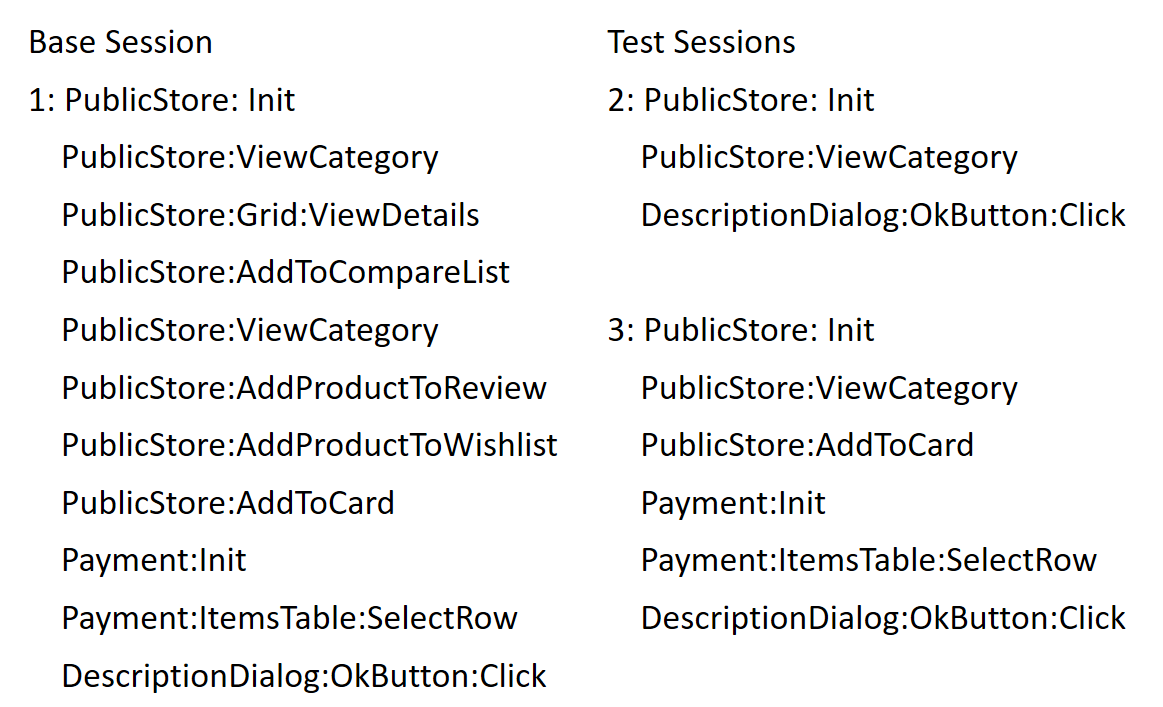
\includegraphics[width=0.90\linewidth]{./SessionSample4.png}
	\caption{Sample of Base Session and Test Sessions}
	\label{fig:sessions}
\end{figure}
	
After collecting all sessions, we conducted an analysis of web forms' access frequency 
by comparing the observed web forms in each session with a base session. 
	
\vspace*{-3pt}
\[
{F_{w,i} = \frac {\sum_{{form\: score\: for \: each\: session}}(S_{i})}
	{\sum_{{number \: of \: base \: sessions}}({BS_{i}})}}	
\]
	
Using Figure~\ref{fig:sessions} as an example, the form ``PublicStore'' 
from the base session was observed in test sessions 2 and 3. 
If we assume that we have ten test sessions and three base sessions,
and this particular form was observed in seven of the ten forms, then the
access frequency of form ``PublicStore'' is equal to $(0.7 / 3) = 0.23$.
	
\subsubsection*{Most Frequent Methods-Based ($T_{mfm}$)}
The most frequent methods approach is nearly identical to the web form frequency technique. 
The only difference is that we considered a method instead of a web form 
as a comparison factor. 
The most frequent methods usually have high dependency on other classes and methods. 
If one of them fails, it can cause a significant failure or degradation of the system. 
In order to prevent a domino effect in the system, high-frequency methods 
should be tested first, because their failure can cause 
other components to fail due to their dependencies.	 	

\subsubsection*{Random ($T_{r}$)}
The random prioritization technique randomly reorders test cases.

\subsubsection*{Greedy ($T_{g}$)}
The greedy technique reorders test cases based on the total number of 
blocks covered by test cases. 

\subsubsection{Dependent Variable} 

Our dependent variable RQ1 is the average percentage of fault detection (APFD)
referring to the average percentage of faults detected during the test suite execution. 
The range of APFD is from 0 to 100, the higher value indicating better prioritization technique. 
Given $T$ as a test suite with $n$ test cases and $m$ number of faults, 
$F$ as a collection of detected faults by $T$, and
$TF_{i}$ as the first test case that catches the fault $i$, 
we calculate APFD ~\cite{apfd} as follows:

\vspace*{-5pt}
%{\scriptsize
\[
{APFD = 1- \frac {{TF_{1} + TF_{2} + ... + TF_{m}}} {nm} + \frac{1}{2n}}
\]
%}
%\vspace*{-5pt}
	
RQ2 seeks to measure the effectiveness of our proposed approach
when we have constrained resources, which means that we need to evaluate 
the effectiveness of our approach using a different metric. 
Qu et al.~\cite{myra} defined the normalized metric of APFD, which is the
area under the curve when the numbers of test cases or faults are not consistent. 
The NAPFD formula is as follows:
	
\vspace*{-5pt}
%{\scriptsize
\[
{NAPFD = p- \frac {{TF_{1} + TF_{2} + ... + TF_{m}}} {nm} + \frac{p}{2n}}
\]
%}
%\vspace*{-5pt}
	
In this formula, $n$ is a percentage of the test suite run, 
$m$ represents the total number of faults found by all test cases,
$TF_{i}$ indicates the same parameter as AFPF, and 
$p$ is the number of faults detected by the percentage of our
budget divided by the total number of detected faults when 
running 100\% of test cases.  

%When evaluating RQ3, the primary concern is how fast test cases reordered 
%by our recommender system can detect all defects in the applications.
%The dependent variable for RQ3 is the total test execution time
%until 100\% defects are detected by each technique.  

\subsection{Data Collection and Experimental Setup}
\label{data-collection}
In order to perform our experiment, for both the control and heuristic techniques
we needed to collect three different types of datasets: telemetry data, change 
history, and code coverage information. We explain the data collection processes
in the following subsections.

\subsubsection{Collection of Telemetry Data}
To collect telemetry data, we implemented a small function to record user interactions. 
We considered a sequence of each user's interactions on a specific date as a user session.
First, we uploaded two applications, {\em Coevery} and {\em nopCommerce}, on an IIS server 
at the University of ABC in November 2016. 
The server specification is CPU Core i7, with 16 GB of RAM.
After deploying our applications, we recruited volunteer graduate and undergraduate
computer science students and assigned a variety of tasks to them. 
These tasks to the volunteers were simple scenarios that each application is designed for.
%%%%%%%% nemidoonammmmmmmmmmmmmmmmmmmmmmmmmmm
For example, in {\em nopCommerce}, we asked the volunteers to perform online shopping 
following the actual necessary steps, from login to payment. We also asked some of 
the users to be the system administrator, so we could monitor the whole system 
rather than only the end user side.
We asked the end users to access other part of the system randomly, for example,
checking their inbox or wish list.  
In total, seventy volunteer students performed different tasks during a forty-day period.  
%%% revierw question
We collected 1,310 and 274 user sessions for {\em nopCommerce}, 
and {\em Coevery} respectively. 
%%%%
 
The data collection process for {\em DASCP} is different from that of {\em Coevery} 
and {\em nopCommerce}. {\em DASCP} is a commercial and closed source application 
that has three versions, and it has been installed on the servers of three companies since 2011. 
The DASCP users whose data we examined are real users, and they have application domain knowledge.
We collected a twelve-month period of user interactions for DASCP.
As described in Section~\ref{sec:objects}, DASCP provides two types of access rights for users.
In this study, we only considered the sessions of those users who have full access to the system.
In total, 748 user sessions were collected during the designated period of time. 

%%% more details about sessions
However, the length of the sessions varied by user, date, and workplace.
For example, some users performed all their assigned task a few hours before the
determined deadline, while others distributed their tasks over several days.
The average length of user sessions for {\em nopCommerce} is equal to 56 and, for
{\em Coevery}, 24. However, in some case we obtained session lengths over 
300, especially when the interaction date was close to the deadline. 
Also, most of the {\em Coevery} users were selected among graduate students, since the
functionality of this application is relatively more complex that of {\em nopCommerce}. 

Figure~\ref{fig:SampleSession3} shows an example of the raw telemetry data. 
The left-hand column shows the session identifier, which is a user
navigating through the system. The right-hand column is the set of server-side user 
interactions. The structure of the interactions is of the format (Form name):(Control name):(Action name).

\begin{figure}[!ht]
\vspace*{-3pt}
	\centering
	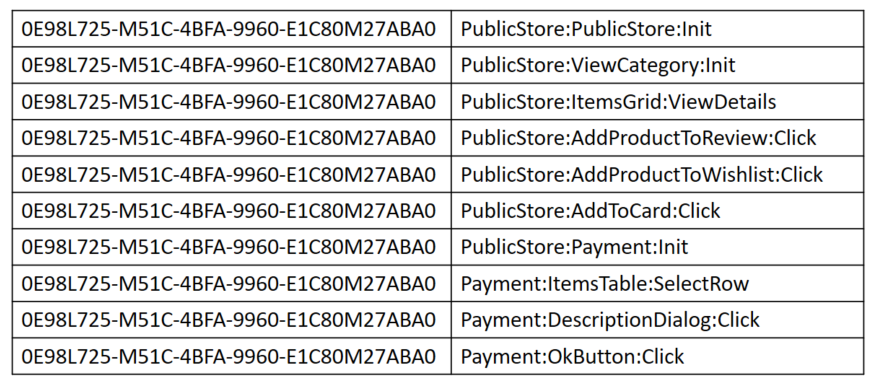
\includegraphics[width=0.90\linewidth]{./SessionSample3.png}
	\caption{Sample User Session}
	\label{fig:SampleSession3}
\end{figure}


\subsubsection{Collection of Code Change History}
We had to take three steps to measure change risk. 
First, we needed a clear understanding of the applications with respect to their changes.
For instance, we needed to check whether a change 
was just the renaming a variable or component, the addition of some comments, 
or an alteration of code by adding or deleting functions, and so on. 
Then, we needed to check whether changes had been made in the current version, 
and finally, we tested a recently changed system~\cite{change3}. 
%In order to collect change history information for training, 
%we used 23 versions of {\em nopCommerece}  and all available versions 
%of our two other applications. 
Figure~\ref{fig:versions} shows the versions that we used in this study. 
%%%%%% not sureeeeeeeeee
{\em nopCommerece} contains 36 versions but we used only the
versions available on the ~\textit{GitHub} repository as of the experiment date. However, for
{\em Coevery} and {\em DASCP}, we used all available versions. 
All studied applications contain fine-grained changes, and the commits on these two open source
applications are available in the \textit{GitHub} repository.   

\begin{figure}[!ht]
	\centering
	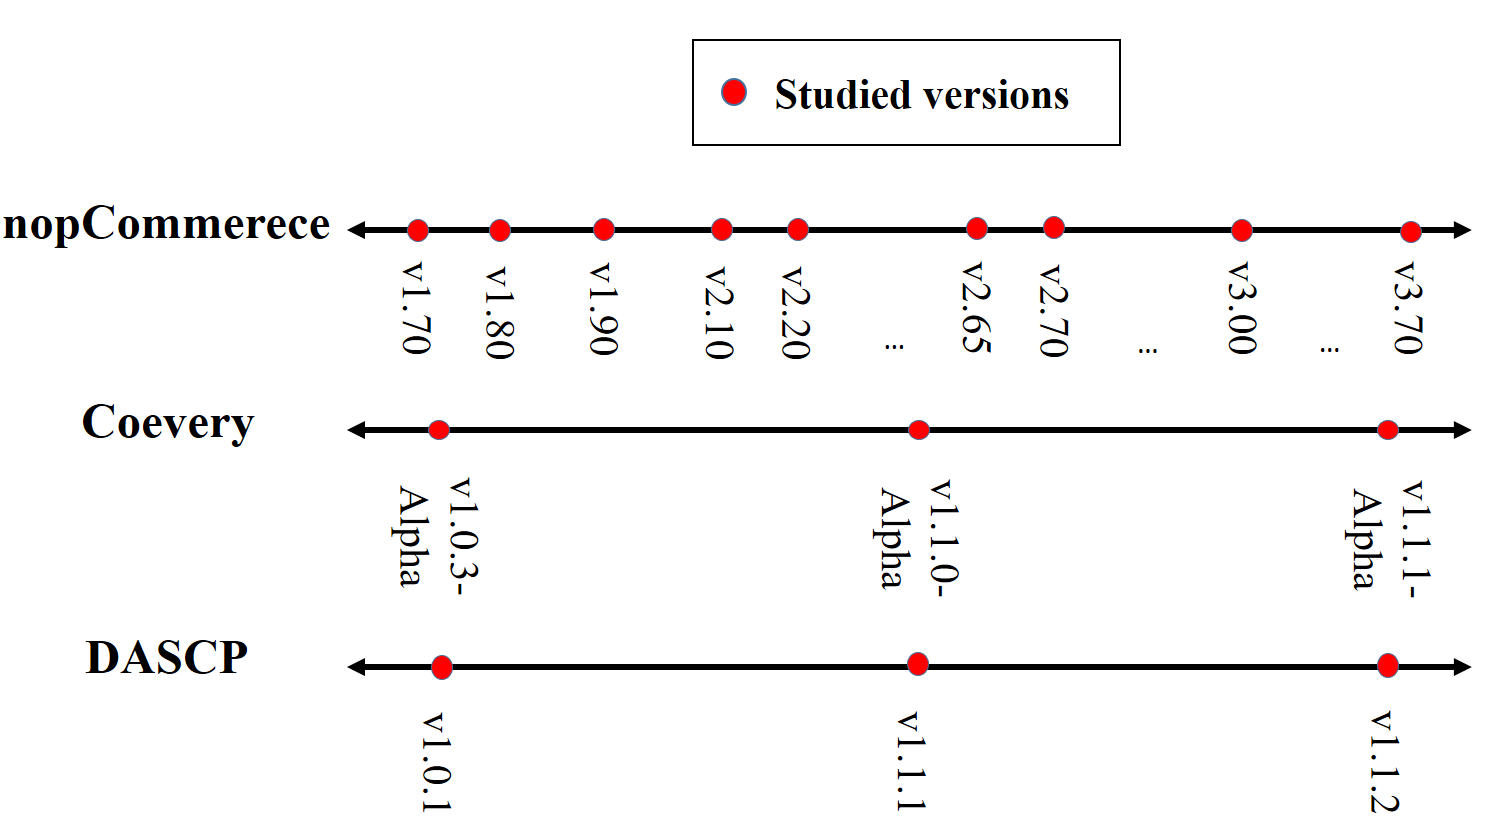
\includegraphics[width=0.95\linewidth]{./Versions2.png}
	\vspace*{-7pt}
	\caption{Versions of Each Application with Change Information and Bug Reports}
	\label{fig:versions}
%	\vspace*{-10pt}
\end{figure}\textbf{}

In our study, we collected the change history of our three applications 
following Giger et al.'s approach ~\cite{method}. 
%We chose ten metrics that have high correlations with bugs.
Most of these metrics have been used in bug detection research, and they
are known to be good indicators for locating bugs~\cite{sungmicro, shihab12, 
raimund, change1, change2, method}.
Table~\ref{tab:historyMetrics} shows the applied change metrics in this study. 

\begin{table}[!ht]
\caption{Change Metrics Used to Evaluate Risk}	
\vspace*{-3pt}
%\begin{tabular*} {.8\linewidth}{@{\extracolsep{\fill}}l|l|}
\begin{tabular} {|l|l|} \hline
	\textbf{Metrics Name} & \textbf{Description} \\\hline \hline
	Modification & Number of times a method was changed  \\\hline
	\multirow{2}{*}{LOC Added} & \parbox[t]{5.5cm}{Added lines of code to a  method \\ body over all method histories} \\\hline
	\multirow{2}{*}{Max LOC Added} & \parbox[t]{5.5cm}{Maximum added lines of code to a method \\ body for all method histories}\\\hline
	\multirow{2}{*}{AVE LOC Added}  & \parbox[t]{5.5cm}{Average added lines of code to a method \\ body per method history}\\\hline
	\multirow{2}{*}{LOC Deleted}  & \parbox[t]{5cm}{Deleted lines of code from a method \\ body over all method histories} \\\hline
	\multirow{2}{*}{Max LOC Deleted} & \parbox[t]{5cm}{Maximum deleted lines from a method \\ body for all method histories}\\\hline
	\multirow{2}{*}{AVE LOC Deleted} & \parbox[t]{5cm}{Average deleted lines from a method \\ body per method history}\\\hline
	Code Churn & Sum of all changes over all method histories\\\hline
	Max Code Churn & Maximum code churn for all method histories \\\hline
	AVE Code Churn & Average code churn  per method history\\\hline
	Age & \parbox[t]{5cm}{Age of a method in weeks from last release} \\\hline
\end{tabular}
\label{tab:historyMetrics}
\vspace*{-6pt}
\end{table}

\subsubsection{Collect Code Coverage}
\label{codecoverage}
Once our recommender system was designed and implemented, 
we needed to find test cases that covered the recommended components. 
We collected the code coverage data for our test cases using the code coverage analysis tool  
that Microsoft Visual Studio provides as part of its framework. 
After collecting the code coverage information, 
we entered it into a relational database. We assigned unique
identifier values for each method and test case, which provides
a key for method and test tables. Hence, we could easily map the methods
to the test cases that exercise them.  

 
\begin{table}[!ht]
\caption{Code Coverage Data Table}
\vspace*{-10pt}
\begin{center}
\begin{tabular}{|c|c|c|c|c|c|} \hline
	MethodID  & Risk Score & TestID1 & ... & TestID n \\\hline
	12 & 0.876 & 0 &  & 0 \\\hline
	287 & 0.012 & 1 &  & 0 \\\hline
	301 & 0.547 & 0 &  & 0 \\\hline
	148 & 0.145 & 0 &  & 1 \\\hline
	67 & 0.055 & 1 &  & 0 \\\hline			
\end{tabular}
\end {center}
\label{tab:coverage}
\vspace*{-10pt}
\end{table}

	
Table~\ref{tab:coverage} show the code coverage data we collected.
The first column, ``MethodID'', shows
the unique identifier values that we assigned for each method. 
The second column shows the final risk scores, which is the output of 
our recommender system. Other columns list our test cases
with Boolean values: 0 indicates that the test case does not cover 
the method, and 1 indicates that the test case covers the method.

\subsubsection{Faults}
\label{faultsInfo}

The applications contain real defects reported by users, but the number of 
defects is rather small considering the size of the applications we studied.
Thus, two graduate students seeded additional faults by simulating  programmers' 
common mistakes (e.g., using a single equal sign to check equality).
All seeded faults were in the server-side code level, and we ignored HTML-based and GUI faults. 
Four types of faults were seeded: (1) data faults that are related to interaction with 
the data store; (2) logic faults that are logic errors in the code; (3) action faults that modify 
parameter values and actions; and (4) linkage faults that change the hyperlinks references.  
Table~\ref{tab:AUTs} shows the total number of faults that including both real and 
seeded faults. The number of real faults for {\em nopCommerce}, {\em Coevery}, and 
{\em DASCP} is 25, 8, and 13, respectively. Once we collected all the required data, 
we ran control and heuristic 
techniques and calculated all the dependent values for the reordered test cases.

